%!TEX root = ./template-skripsi.tex

\subsection{Sprint 10 Report}
Berikut merupakan report dari sprint ke-10 yang dilakukan pada tanggal 20 juli - 26 juli 2022.

\begin{table}[H]
	\caption{\textit{Sprint-10 backlog}}
	\label{sprint10_backlog}
	\begin{tabular}{@{} |p{0.5cm}|p{5cm}|p{5cm}|p{2cm}| @{}}
		\hline
		\textbf{No} & \textbf{\textit{Story}} & \textbf{\textit{Task}} & \textbf{\textit{Status}} \\
		\hline
		1 & \multirow{3}{5cm}{Create, Read, Updte, dan Delete untuk Treatment kolam} & Membarui desain database  & Completed\\
		\cline{1-1}\cline{3-4}
		2 & & Menambahkan routes API & Completed\\
		\cline{1-1}\cline{3-4}
		3 & & Implementasi controller entry treatment kolam & Completed\\
		\cline{1-1}\cline{3-4}
		4 & & Implementasi controller fetch list treatment kolam & Completed\\
		\cline{1-1}\cline{3-4}
		5 & & Implementasi controller edit treatment kolam & Completed\\
		\cline{1-1}\cline{3-4}
		6 & & Implementasi controller delete treatment kolam & Completed\\
		\cline{1-1}\cline{3-4}
		7 & & Implementasi controller fetch detail treatment kolam dengan id& Completed\\
		\cline{1-1}\cline{3-4}
		8 & & Membuat view rekap treatment kolam & Completed\\
		\cline{1-1}\cline{3-4}
		\hline
	\end{tabular}
\end{table}

\begin{enumerate}[1.]

\item \textbf{Membarui desain database}

\begin{figure}[H]
	\centering
	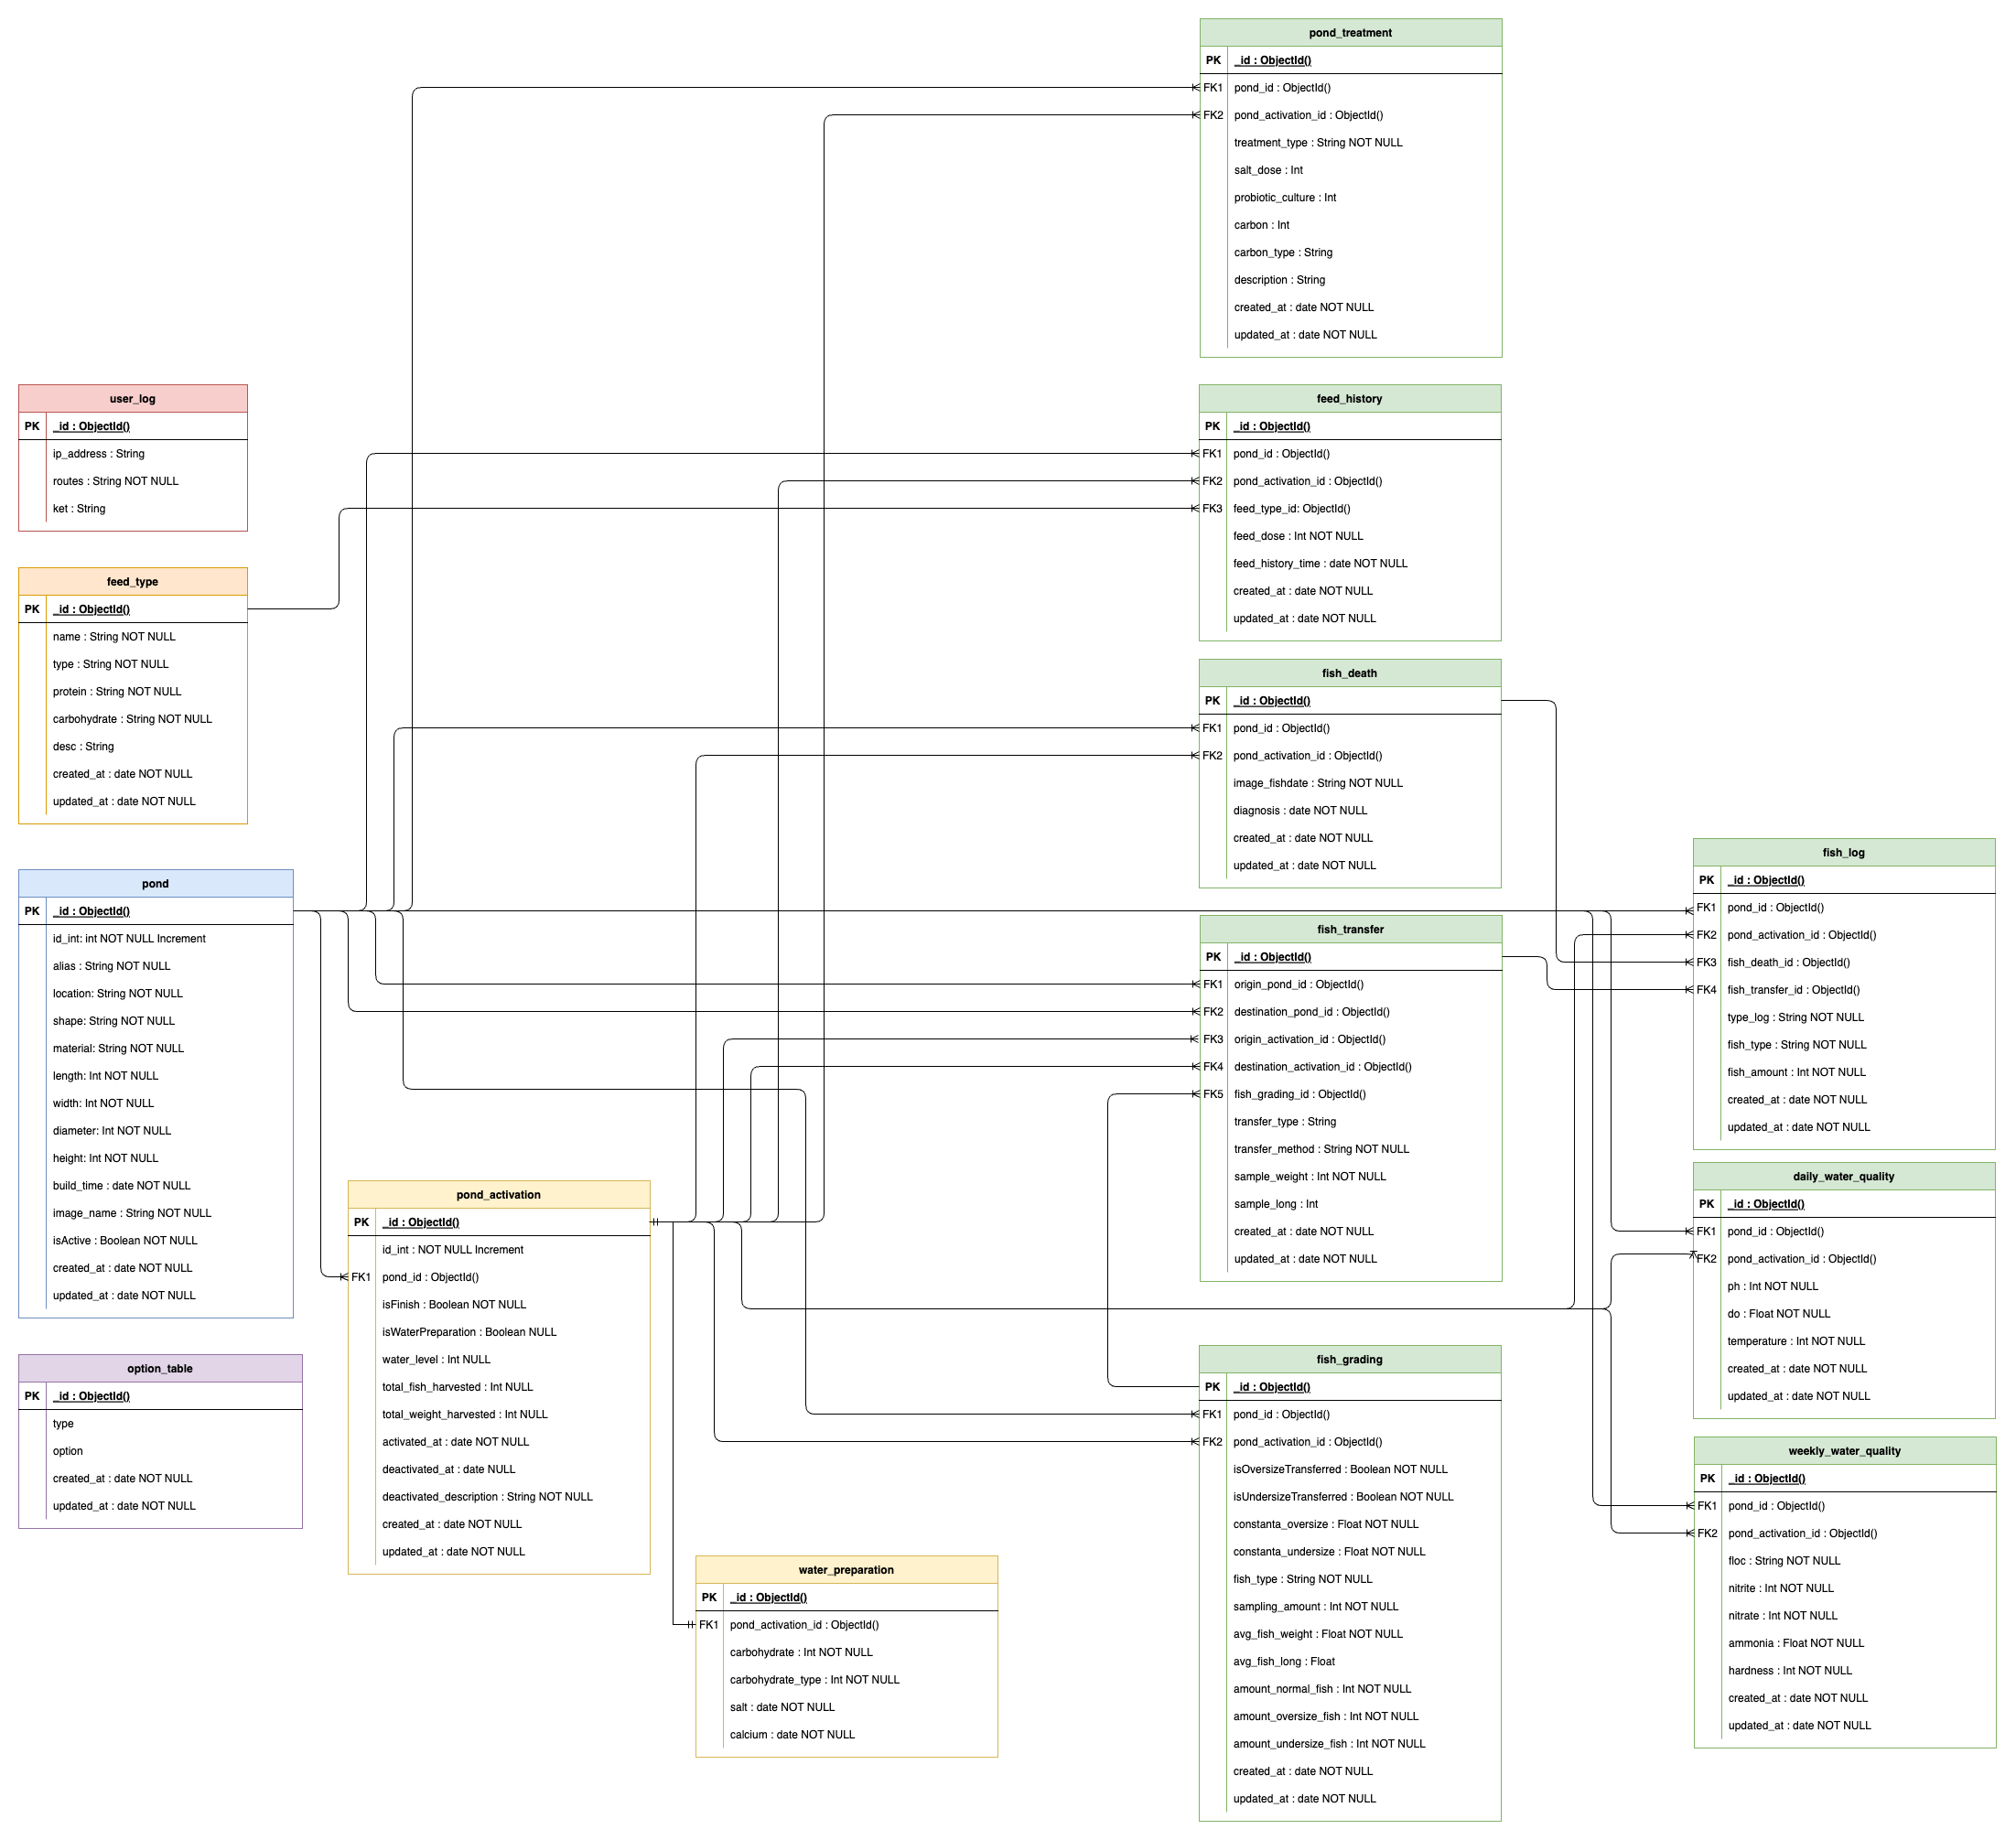
\includegraphics[height=0.7\textwidth]{gambar/Sprint10/diagram database/database}
	\caption{ERD Database Sprint-10}
	\label{fig:database_sprint10}
\end{figure}

Dengan berubahnya desain database diperlukan juga penambahan model pada source code, berikut perubahan pada source code model.

\begin{lstlisting}
# fishapi/database/model.py

class PondTreatment(db.Document):
    treatment_type_option = ("ringan", "karantina", "pergantian air")
    carbohydrate_type_option = ("", "gula", "molase", "terigu", "tapioka")

    pond_id = db.ReferenceField(Pond, required=True)
    pond_activation_id = db.ReferenceField(PondActivation, required=True)
    treatment_type = db.StringField(required=True, choices=treatment_type_option)
    water_change = db.IntField()
    salt = db.IntField()
    probiotic_culture = db.IntField()
    carbohydrate = db.IntField()
    carbohydrate_type = db.StringField(required=True, choices=carbohydrate_type_option, default="")
    description = db.StringField(default="")
    created_at = db.DateTimeField(default=datetime.datetime.now)
    updated_at = db.DateTimeField(default=datetime.datetime.now)
\end{lstlisting}



\item \textbf{Menambahkan routes API}

\begin{lstlisting}
# fishapi/resource/routes.py

# pond treatment
    api.add_resource(PondTreatmentsApi, '/api/pondtreatment')
    api.add_resource(PondTreatmentApi, '/api/pondtreatment/<id>')
\end{lstlisting}




\item \textbf{Implementasi controller entry treatment kolam}

Implementasi controller API entry treatment kolam, berikut merupakan perubahan source code controller API entry treatment kolam.

\begin{lstlisting}
# fishapi/resource/pondtreatment.py

class PondTreatmentsApi(Resource):
    def post(self):
        try:
            pond_id = request.form.get("pond_id", None)
            pond = Pond.objects.get(id=pond_id)
            if pond['isActive'] == False:
                response = {"message": "pond is not active"}
                response = json.dumps(response, default=str)
                return Response(response, mimetype="application/json", status=400)
            pond_activation = PondActivation.objects(
                pond_id=pond_id, isFinish=False).order_by('-activated_at').first()
            treatment_type = request.form.get("treatment_type", None)
            if treatment_type == "karantina":
                body = {
                    "pond_id": pond_id,
                    "pond_activation_id": pond_activation.id,
                    "treatment_type": treatment_type,
                    "water_change": 100,
                    "description": request.form.get("description", None),
                }
                pondtreatment = PondTreatment(**body).save()
                id = pondtreatment.id
                # update activation and pond
                pond_deactivation_data = {
                    "isFinish": True,
                    "total_fish_harvested": request.form.get("total_fish_harvested", None),
                    "total_weight_harvested": request.form.get("total_weight_harvested", None),
                    "deactivated_at": request.form.get("deactivated_at", datetime.datetime.now()),
                    "deactivated_description": "karantina total"
                }
                pond_activation = PondActivation.objects(
                    pond_id=pond_id, isFinish=False).order_by('-activated_at').first()
                pond_activation.update(**pond_deactivation_data)
                pond.update(**{"isActive": False})
            elif treatment_type == "ringan":
                body = {
                    "pond_id": pond_id,
                    "pond_activation_id": pond_activation.id,
                    "treatment_type": treatment_type,
                    "water_change": 0,
                    "salt": request.form.get("salt_dose", None),
                    "probiotic_culture": request.form.get("probiotic_culture", None),
                    "carbohydrate": request.form.get("carbohydrate", None),
                    "carbohydrate_type": request.form.get("carbohydrate_type", None),
                }
                pondtreatment = PondTreatment(**body).save()
                id = pondtreatment.id
            elif treatment_type == "pergantian air":
                body = {
                    "pond_id": pond_id,
                    "pond_activation_id": pond_activation.id,
                    "treatment_type": treatment_type,
                    "water_change": request.form.get("water_change", 0)
                }
                pondtreatment = PondTreatment(**body).save()
                id = pondtreatment.id
            else:
                response = {
                    "message": "treatment type just allow ['ringan','berat']"}
                response = json.dumps(response, default=str)
                return Response(response, mimetype="application/json", status=400)
            response = {
                "message": "success add data pond treatment", "id": id}
            response = json.dumps(response, default=str)
            return Response(response, mimetype="application/json", status=200)
        except Exception as e:
            response = {"message": str(e)}
            response = json.dumps(response, default=str)
            return Response(response, mimetype="application/json", status=400)
\end{lstlisting}

Kode di atas adalah implementasi sebuah API untuk menangani permintaan POST pada endpoint PondTreatmentsApi.

Pertama, kode tersebut mengambil nilai pond\_id dari formulir permintaan menggunakan request.form.get("pond\_id", None). Kemudian, dilakukan pencarian objek Pond berdasarkan pond\_id yang diperoleh.

Selanjutnya, dilakukan pengecekan apakah kolom isActive pada objek Pond memiliki nilai False. Jika iya, maka dikembalikan respons dengan pesan "pond is not active" dan status kode 400.

Selanjutnya, dilakukan pencarian objek PondActivation berdasarkan pond\_id dan isFinish=False dengan pengurutan berdasarkan activated\_at secara menurun menggunakan .order\_by('-activated\_at').first(). Nilai treatment\_type juga diambil dari formulir permintaan.

Kemudian, dilakukan pengecekan terhadap treatment\_type. Jika nilainya adalah "karantina", maka dibentuk sebuah body yang berisi data-data untuk membuat objek PondTreatment dengan beberapa nilai yang diambil dari formulir permintaan. Objek PondTreatment tersebut kemudian disimpan ke database menggunakan .save(). Nilai id dari objek tersebut diambil untuk digunakan sebagai respons.

Selanjutnya, dilakukan pembaruan (update) pada objek PondActivation dan Pond. Data-data yang diperbarui disimpan dalam variabel pond\_deactivation\_data dan pond\_activation yang merupakan objek PondActivation terakhir yang ditemukan. Objek-objek tersebut diupdate menggunakan .update().

Jika treatment\_type adalah "ringan", maka langkah yang serupa dilakukan untuk membentuk objek PondTreatment dengan data yang sesuai.

Jika treatment\_type adalah "pergantian air", maka juga dilakukan langkah yang serupa untuk membentuk objek PondTreatment dengan data yang sesuai.

Jika treatment\_type tidak sesuai dengan ketiga opsi yang diberikan ("karantina", "ringan", "pergantian air"), maka dikembalikan respons dengan pesan "treatment type just allow ['ringan','berat']" dan status kode 400.

Terakhir, jika tidak terjadi kesalahan, respons berhasil dibentuk dengan pesan "success add data pond treatment" dan nilai id dari objek PondTreatment yang telah dibuat. Respons tersebut dikonversi menjadi JSON dan dikembalikan dengan tipe konten "application/json" dan status kode 200. Jika terjadi kesalahan, tangkapan Exception akan menghasilkan pesan kesalahan yang dikirim sebagai respons dengan status kode 400.

Berikut merupakan form untuk entry grading berat ikan antar kolam.

\begin{longtable}{| l | p{5cm} | p{5cm} |}
\caption{Form entry treatment kolam.\label{table:form_entry_treatment_kolam}}\\

\hline
\multicolumn{1}{|c|}{\textbf{Form}} & \multicolumn{1}{|c|}{\textbf{Jenis Data}} & \multicolumn{1}{|c|}{\textbf{Deskripsi}}\\
\hline
\endfirsthead

\hline
\multicolumn{3}{|c|}{Lanjutan Tabel \ref{table:form_entry_treatment_kolam}}\\
\hline
\multicolumn{1}{|c|}{\textbf{Form}} & \multicolumn{1}{|c|}{\textbf{Jenis Data}} & \multicolumn{1}{|c|}{\textbf{Deskripsi}}\\
\hline
\endhead

                                          

pond\_id                 & REQUIRED STRING                                                                                          & id kolam yang akan di lakukan treatment                                      \\ \hline
treatment\_type          & REQUIRED STRING VALUE : {[}"ringan", "karantina", "pergantian air" {]}                                   & tipe treatment yang akan dilakukan                                           \\ \hline
salt                     & OPTIONAL INT                                                                                             & takaran penambahan garam ke kolam dalam satuan gram                          \\ \hline
probiotic\_culture       & OPTIONAL INT                                                                                             & takaran penambahan probiotik ke kolam dalam satuan gram                      \\ \hline
carbohydrate             & OPTIONAL INT                                                                                             & takaran penambahan zat karbon ke kolam dalam satuan gram                     \\ \hline
carbohydrate\_type       & REQUIRED IF "carbohydrate" \textgreater 0 STRING VALUE : {[}"", "gula", "molase", "terigu", "tapioka"{]} & tipe zat karbon                                                              \\ \hline
description              & OPTIONAL STRING                                                                                          & keterangan treatment kolam                                                   \\ \hline
total\_fish\_harvested   & REQUIRED IF "treatment\_type" == "karantina" INT                                                         & jumlah ikan yang di panen pada saat kolam di karantina                       \\ \hline
total\_weight\_harvested & REQUIRED IF "treatment\_type" == "karantina" INT                                                         & jumlah berat ikan yang di panen pada saat kolam di karantina dalam satuan Kg \\ \hline
water\_change            & REQUIRED IF "treatment\_type" == "pergantian air" INT                                                    & persentase pergantian air pada kolam                                         \\ \hline
\end{longtable}



Tabel di atas merupakan daftar parameter yang dapat digunakan dalam formulir permintaan (request form) pada API PondTreatmentsApi. Setiap kolom dalam tabel memiliki informasi yang relevan terkait jenis data yang diharapkan dan deskripsi dari parameter tersebut. Berikut adalah penjelasan dari setiap kolom:

\begin{enumerate}
\item pond\_id: Parameter ini harus diisi dengan tipe data STRING yang wajib ada. Parameter ini digunakan untuk mengidentifikasi kolam yang akan diberikan treatment.

\item treatment\_type: Parameter ini harus diisi dengan tipe data STRING yang wajib ada. Nilai yang dapat diterima adalah "ringan", "karantina", atau "pergantian air". Parameter ini menentukan jenis treatment yang akan dilakukan pada kolam.

\item salt: Parameter ini bersifat opsional dan harus diisi dengan tipe data INT. Parameter ini digunakan untuk menentukan takaran penambahan garam ke dalam kolam dalam satuan gram.

\item probiotic\_culture: Parameter ini bersifat opsional dan harus diisi dengan tipe data INT. Parameter ini digunakan untuk menentukan takaran penambahan probiotik ke dalam kolam dalam satuan gram.

\item carbohydrate: Parameter ini bersifat opsional dan harus diisi dengan tipe data INT. Parameter ini digunakan untuk menentukan takaran penambahan zat karbon ke dalam kolam dalam satuan gram.

\item carbohydrate\_type: Parameter ini harus diisi jika nilai dari "carbohydrate" lebih besar dari 0. Parameter ini harus diisi dengan tipe data STRING. Nilai yang dapat diterima adalah "", "gula", "molase", "terigu", atau "tapioka". Parameter ini menentukan jenis zat karbon yang ditambahkan.

\item description: Parameter ini bersifat opsional dan harus diisi dengan tipe data STRING. Parameter ini digunakan untuk memberikan keterangan tambahan mengenai treatment kolam.

\item total\_fish\_harvested: Parameter ini harus diisi jika "treatment\_type" memiliki nilai "karantina". Parameter ini harus diisi dengan tipe data INT. Parameter ini menentukan jumlah ikan yang dipanen saat kolam dalam kondisi karantina.

\item total\_weight\_harvested: Parameter ini harus diisi jika "treatment\_type" memiliki nilai "karantina". Parameter ini harus diisi dengan tipe data INT. Parameter ini menentukan jumlah berat ikan yang dipanen saat kolam dalam kondisi karantina, dalam satuan kilogram.

\item water\_change: Parameter ini harus diisi jika "treatment\_type" memiliki nilai "pergantian air". Parameter ini harus diisi dengan tipe data INT. Parameter ini menentukan persentase pergantian air pada kolam.
\end{enumerate}

Tabel ini memberikan panduan yang berguna dalam menggunakan API PondTreatmentsApi dengan benar, menunjukkan parameter apa yang harus disertakan dalam permintaan dan jenis data yang diharapkan untuk setiap parameter tersebut.


Berikut merupakan hasil test request dari API entry treatment kolam.

cURL:

\begin{lstlisting}
curl --location 'http://jft.web.id/fishapi/api/pondtreatment' \
--form 'pond_id="{pond_id}"' \
--form 'treatment_type="karantina"' \
--form 'description="penyakit ikan sekolam"'
\end{lstlisting}

response json:

\begin{lstlisting}
{
  "message": "success add data pond treatment",
  "id": "62f5248cae2842f914ee7797"
}
\end{lstlisting}




\item \textbf{Implementasi API fetch list treatment kolam}

Implementasi controller API fetch list treatment kolam, berikut merupakan source code controller API fetch list treatment kolam.

\begin{lstlisting}
# fishapi/resource/pondtreatment.py

def get(self):
        try:
            pipeline = [
                {"$sort": {"created_at": 1}},
                {'$lookup': {
                    'from': 'pond',
                    'let': {"pondid": "$pond_id"},
                    'pipeline': [
                        {'$match': {'$expr': {'$eq': ['$_id', '$$pondid']}}},
                        {"$project": {
                            "_id": 1,
                            "alias": 1,
                            "location": 1,
                            "build_at": 1,
                            "isActive": 1,
                        }}
                    ],
                    'as': 'pond'
                }},
                {'$lookup': {
                    'from': 'pond_activation',
                    'let': {"activationid": "$pond_activation_id"},
                    'pipeline': [
                        {'$match': {
                            '$expr': {'$eq': ['$_id', '$$activationid']}}},
                        {"$project": {
                            "_id": 1,
                            "isFinish": 1,
                            "isWaterPreparation": 1,
                            "water_level": 1,
                            "activated_at": 1
                        }}
                    ],
                    'as': 'pond_activation'
                }},
                {"$addFields": {
                    "pond": {"$first": "$pond"},
                    "pond_activation": {"$first": "$pond_activation"},
                }},
                {"$project": {
                    "updated_at": 0,
                    "created_at": 0,
                }}
            ]
            pondtreatment = PondTreatment.objects.aggregate(pipeline)
            list_pondtreatments = list(pondtreatment)
            response = json.dumps(list_pondtreatments, default=str)
            return Response(response, mimetype="application/json", status=200)
        except Exception as e:
            response = {"message": str(e)}
            response = json.dumps(response, default=str)
            return Response(response, mimetype="application/json", status=400)
\end{lstlisting}



Kode di atas merupakan implementasi metode get() dalam sebuah class yang mengatur API. Metode ini digunakan untuk mengambil data PondTreatment (pengobatan kolam) dari database menggunakan agregasi dengan pipeline MongoDB. Berikut adalah penjelasan langkah-langkah yang dilakukan oleh kode tersebut:

\begin{enumerate}
\item Sebuah pipeline MongoDB dibuat untuk mengatur tahapan-tahapan pemrosesan data.
\item Pada tahap pertama, data akan diurutkan berdasarkan waktu pembuatan (created\_at) secara ascending (1).
\item Tahap berikutnya adalah melakukan operasi \$lookup untuk melakukan join (penggabungan) dengan koleksi pond. Tahap ini menggabungkan data \item PondTreatment dengan data kolam yang sesuai berdasarkan pond\_id. Hasil join ini akan mencakup proyeksi hanya beberapa field yang spesifik.
\item Selanjutnya, dilakukan operasi \$lookup kedua untuk melakukan join dengan koleksi pond\_activation. Tahap ini menggabungkan data PondTreatment dengan data aktivasi kolam yang sesuai berdasarkan pond\_activation\_id. Seperti sebelumnya, hasil join ini juga mencakup proyeksi hanya beberapa field yang spesifik.
\item Setelah join, dilakukan operasi \$addFields untuk menambahkan dua field baru, yaitu pond dan pond\_activation. Nilai dari kedua field ini diambil dari elemen pertama dalam array hasil join.
\item Tahap selanjutnya adalah operasi \$project yang digunakan untuk mengatur proyeksi output, dalam hal ini menghilangkan field updated\_at dan created\_at.
\item Setelah pipeline terbentuk, pipeline ini digunakan untuk melakukan agregasi pada koleksi PondTreatment menggunakan metode aggregate(). Hasil agregasi ini akan berupa kursor MongoDB.
\item Kursor hasil agregasi diubah menjadi list dengan menggunakan fungsi list().
\item Hasil list PondTreatment yang sudah diubah ke dalam format JSON menggunakan json.dumps().
\item Hasil akhir dikembalikan sebagai respons dengan tipe Response yang memiliki tipe konten "application/json" dan status kode 200.
\item Jika terjadi exception atau kesalahan, akan di-handle dengan mengembalikan respons dengan pesan error yang sesuai dalam format JSON dan status kode 400.
\end{enumerate}
Dengan demikian, kode tersebut melakukan proses pengambilan data PondTreatment dari database menggunakan agregasi dengan pipeline, menggabungkan data dengan koleksi lain, dan mengatur format dan status respons yang dihasilkan.

Berikut merupakan hasil test request dari API fetch list treatment kolam.

cURL:

\begin{lstlisting}
curl --location 'http://jft.web.id/fishapi/api/pondtreatment'
\end{lstlisting}

response json:

\begin{lstlisting}
[
  {
    "_id": "62f5248cae2842f914ee7797",
    "pond_id": "62a62163e445ffb9c5f746f3",
    "pond_activation_id": "62d3f2180d7265ab60f9cb83",
    "treatment_type": "ringan",
    "probiotic_culture": 10,
    "carbohydrate": 10,
    "carbohydrate_type": "gula",
    "pond": {
      "_id": "62a62163e445ffb9c5f746f3",
      "alias": "charlie",
      "location": "blok 2",
      "build_at": "2022-06-13 00:24:51.473000",
      "isActive": false
    },
    "pond_activation": {
      "_id": "62d3f2180d7265ab60f9cb83",
      "isFinish": true,
      "isWaterPreparation": true,
      "water_level": 100,
      "activated_at": "2022-07-17 18:27:20.511000"
    }
  },
  {
    "_id": "62f52c34307b0c2008380309",
    "pond_id": "62a62163e445ffb9c5f746f3",
    "pond_activation_id": "62d3f2180d7265ab60f9cb83",
    "treatment_type": "karantina",
    "carbohydrate_type": "",
    "description": "penyakit ikan sekolam",
    "pond": {
      "_id": "62a62163e445ffb9c5f746f3",
      "alias": "charlie",
      "location": "blok 2",
      "build_at": "2022-06-13 00:24:51.473000",
      "isActive": false
    },
    "pond_activation": {
      "_id": "62d3f2180d7265ab60f9cb83",
      "isFinish": true,
      "isWaterPreparation": true,
      "water_level": 100,
      "activated_at": "2022-07-17 18:27:20.511000"
    }
  }
]
\end{lstlisting}



\item \textbf{Implementasi API edit treatment kolam}

Implementasi controller API edit treatment kolam, berikut merupakan perubahan source code controller API edit treatment kolam.

\begin{lstlisting}
# fishapi/database/pondtreatment.py

def put(self, id):
        try:
            body = request.form.to_dict(flat=True)
            PondTreatment.objects.get(id=id).update(**body)
            response = {
                "message": "success change data pond treatment", "id": id}
            response = json.dumps(response, default=str)
            return Response(response, mimetype="application/json", status=200)
        except Exception as e:
            response = {"message": str(e)}
            response = json.dumps(response, default=str)
            return Response(response, mimetype="application/json", status=400)
\end{lstlisting}

Kode di atas merupakan implementasi metode put() dalam sebuah modul pondtreatment.py yang berfungsi untuk memperbarui data PondTreatment (pengobatan kolam) dalam database. Berikut adalah penjelasan langkah-langkah yang dilakukan oleh kode tersebut:

\begin{enumerate}
\item Metode put() menerima parameter id yang merupakan identifikasi unik dari PondTreatment yang akan diperbarui.
\item Di dalam blok try, pertama-tama dilakukan pengambilan data dari form request menggunakan request.form.to\_dict(flat=True). Data tersebut dikonversi menjadi bentuk dictionary dengan argumen flat=True.
\item Selanjutnya, menggunakan metode get() dari PondTreatment.objects dengan memanfaatkan id yang diberikan, data PondTreatment yang sesuai diambil dari database.
\item Data PondTreatment tersebut kemudian diperbarui menggunakan metode update() dengan argumen **body, yang berarti data pada field-field yang sesuai dalam PondTreatment akan diperbarui dengan nilai baru dari body (dictionary yang berisi data dari form request).
\item Setelah proses pembaruan selesai, respons berhasil dengan pesan success dan id PondTreatment yang telah diperbarui dibuat.
\item Respons tersebut diubah menjadi format JSON menggunakan json.dumps().
\item Hasil akhir dikembalikan sebagai respons dengan tipe Response yang memiliki tipe konten "application/json" dan status kode 200.
\item Jika terjadi exception atau kesalahan, akan di-handle dengan mengembalikan respons dengan pesan error yang sesuai dalam format JSON dan status kode 400.
\end{enumerate}
Dengan demikian, kode tersebut melakukan proses pembaruan data PondTreatment dengan menggunakan data yang diterima dari form request. Data PondTreatment diambil dari database menggunakan get() dan kemudian diperbarui dengan nilai baru. Respons yang dihasilkan mengindikasikan keberhasilan pembaruan atau kesalahan yang terjadi.

Berikut merupakan hasil test request dari API edit treatment kolam.

cURL:

\begin{lstlisting}
curl --location --request PUT 'http://jft.web.id/fishapi/api/pondtreatment/62f5248cae2842f914ee7797' \
--form 'salt="20"' \
--form 'probiotic_culture="20"' \
--form 'carbohydrate="20"' \
--form 'carbohydrate_type="molase"'
\end{lstlisting}

response json:

\begin{lstlisting}
{
  "message": "success change data pond treatment",
  "id": "62f5248cae2842f914ee7797"
}
\end{lstlisting}



\item \textbf{Implementasi API delete treatment kolam}

Implementasi controller API delete treatment kolam, berikut merupakan perubahan source code controller API delete treatment kolam.

\begin{lstlisting}
# fishapi/database/pondtreatment.py

def delete(self, id):
        try:
            pondtreatment = PondTreatment.objects.get(id=id).delete()
            response = {"message": "success delete pond treatment"}
            response = json.dumps(response, default=str)
            return Response(response, mimetype="application/json", status=200)
        except Exception as e:
            response = {"message": str(e)}
            response = json.dumps(response, default=str)
            return Response(response, mimetype="application/json", status=400)
\end{lstlisting}


Kode di atas merupakan implementasi metode delete() dalam modul pondtreatment.py yang bertanggung jawab untuk menghapus data PondTreatment (pengobatan kolam) dari database. Berikut adalah penjelasan langkah-langkah yang dilakukan oleh kode tersebut:

Metode delete() menerima parameter id yang merupakan identifikasi unik dari PondTreatment yang akan dihapus. Di dalam blok try, pertama-tama dilakukan pengambilan data PondTreatment dari database menggunakan metode get() dari PondTreatment.objects dengan menggunakan id yang diberikan. Setelah data PondTreatment berhasil diambil, dilakukan penghapusan data tersebut dari database menggunakan metode delete().
Setelah proses penghapusan selesai, respons berhasil dengan pesan success dihasilkan. Respons tersebut diubah menjadi format JSON menggunakan json.dumps(). Hasil akhir dikembalikan sebagai respons dengan tipe Response yang memiliki tipe konten "application/json" dan status kode 200. Jika terjadi exception atau kesalahan, akan di-handle dengan mengembalikan respons dengan pesan error yang sesuai dalam format JSON dan status kode 400.

Dengan demikian, kode tersebut melakukan proses penghapusan data PondTreatment dari database berdasarkan id yang diberikan. Jika penghapusan berhasil, akan mengembalikan respons dengan pesan keberhasilan. Jika terjadi kesalahan, akan mengembalikan respons dengan pesan error yang sesuai.

Berikut merupakan hasil test request dari API delete treatment kolam.

cURL:

\begin{lstlisting}
curl --location --request DELETE 'http://jft.web.id/fishapi/api/pondtreatment/62e8b800ef4edacc5bb18b05'
\end{lstlisting}

response json:

\begin{lstlisting}
{
  "message": "success delete pond treatment"
}
\end{lstlisting}


\item \textbf{Implementasi API fetch detail treatment kolam dengan id}

Implementasi controller API fetch detail treatment kolam, berikut merupakan source code controller API fetch detail treatment kolam.

\begin{lstlisting}
# fishapi/resource/pondtreatment.py

def get(self, id):
        try:
            pipeline = [
                {'$match': {'$expr': {'$eq': ['$_id', {'$toObjectId': id}]}}},
                {'$lookup': {
                    'from': 'pond',
                    'let': {"pondid": "$pond_id"},
                    'pipeline': [
                        {'$match': {'$expr': {'$eq': ['$_id', '$$pondid']}}},
                        {"$project": {
                            "_id": 1,
                            "alias": 1,
                            "location": 1,
                            "build_at": 1,
                            "isActive": 1,
                        }}
                    ],
                    'as': 'pond'
                }},
                {'$lookup': {
                    'from': 'pond_activation',
                    'let': {"activationid": "$pond_activation_id"},
                    'pipeline': [
                        {'$match': {
                            '$expr': {'$eq': ['$_id', '$$activationid']}}},
                        {"$project": {
                            "_id": 1,
                            "isFinish": 1,
                            "isWaterPreparation": 1,
                            "water_level": 1,
                            "activated_at": 1
                        }}
                    ],
                    'as': 'pond_activation'
                }},
                {"$addFields": {
                    "pond": {"$first": "$pond"},
                    "pond_activation": {"$first": "$pond_activation"},
                }},
                {"$project": {
                    "updated_at": 0,
                    "created_at": 0,
                }}
            ]
            pondtreatment = PondTreatment.objects.aggregate(pipeline)
            list_pondtreatments = list(pondtreatment)
            response = json.dumps(list_pondtreatments[0], default=str)
            return Response(response, mimetype="application/json", status=200)
        except Exception as e:
            response = {"message": str(e)}
            response = json.dumps(response, default=str)
            return Response(response, mimetype="application/json", status=400)
\end{lstlisting}


Kode di atas merupakan implementasi metode get() dalam modul pondtreatment.py yang bertanggung jawab untuk mendapatkan data PondTreatment (pengobatan kolam) berdasarkan id yang diberikan dari database. Berikut adalah penjelasan langkah-langkah yang dilakukan oleh kode tersebut:

\begin{enumerate}
\item Metode get() menerima parameter id yang merupakan identifikasi unik dari PondTreatment yang ingin didapatkan.
\item Di dalam blok try, sebuah pipeline MongoDB disusun untuk melakukan agregasi data PondTreatment berdasarkan id yang diberikan.
\item Pipeline ini terdiri dari beberapa tahapan:
\begin{enumerate}
\item Pertama, dilakukan pencocokan (\$match) berdasarkan ekspresi yang membandingkan \_id dengan id yang dikonversi menggunakan \$toObjectId.
\item Selanjutnya, dilakukan operasi \$lookup untuk menggabungkan (join) dengan koleksi "pond". Hasilnya akan disimpan dalam field "pond".
\item Kemudian, dilakukan operasi \$lookup untuk menggabungkan (join) dengan koleksi "pond\_activation". Hasilnya akan disimpan dalam field "pond\_activation".
\item Selanjutnya, menggunakan \$addFields, field "pond" dan "pond\_activation" diatur sebagai nilai pertama (\$first) dari array yang dihasilkan oleh operasi \$lookup, sehingga hanya satu dokumen yang disimpan.
\item Terakhir, menggunakan \$project, field "updated\_at" dan "created\_at" dihilangkan dari hasil akhir.
\end{enumerate}
\item Setelah pipeline selesai, dilakukan agregasi data PondTreatment menggunakan PondTreatment.objects.aggregate() dengan pipeline yang telah disusun.
\item Hasil agregasi kemudian diubah menjadi list menggunakan list().
\item Dalam hal ini, dianggap bahwa hasil agregasi akan menghasilkan satu dokumen PondTreatment. Oleh karena itu, hanya elemen pertama dari list yang diambil.
\item Hasil tersebut diubah menjadi format JSON menggunakan json.dumps().
\item Hasil akhir dikembalikan sebagai respons dengan tipe Response yang memiliki tipe konten "application/json" dan status kode 200.
\item Jika terjadi exception atau kesalahan, akan di-handle dengan mengembalikan respons dengan pesan error yang sesuai dalam format JSON dan status kode 400.
\end{enumerate}

Dengan demikian, kode tersebut melakukan pengambilan data PondTreatment dari database berdasarkan id yang diberikan menggunakan operasi agregasi MongoDB. Jika pengambilan data berhasil, akan mengembalikan respons dengan data PondTreatment dalam format JSON. Jika terjadi kesalahan, akan mengembalikan respons dengan pesan error yang sesuai.


Berikut merupakan hasil test request dari API fetch treatment kolam berdasarkan id.

cURL:

\begin{lstlisting}
curl --location 'http://jft.web.id/fishapi/api/pondtreatment/62f5248cae2842f914ee7797'
\end{lstlisting}

response json:

\begin{lstlisting}
{
  "_id": "62f5248cae2842f914ee7797",
  "pond_id": "62a62163e445ffb9c5f746f3",
  "pond_activation_id": "62d3f2180d7265ab60f9cb83",
  "treatment_type": "ringan",
  "probiotic_culture": 10,
  "carbohydrate": 10,
  "carbohydrate_type": "gula",
  "pond": {
    "_id": "62a62163e445ffb9c5f746f3",
    "alias": "charlie",
    "location": "blok 2",
    "build_at": "2022-06-13 00:24:51.473000",
    "isActive": false
  },
  "pond_activation": {
    "_id": "62d3f2180d7265ab60f9cb83",
    "isFinish": true,
    "isWaterPreparation": true,
    "water_level": 100,
    "activated_at": "2022-07-17 18:27:20.511000"
  }
}
\end{lstlisting}

\item \textbf{Membuat view rekap treatment kolam}
\begin{figure}[H]
	\centering
	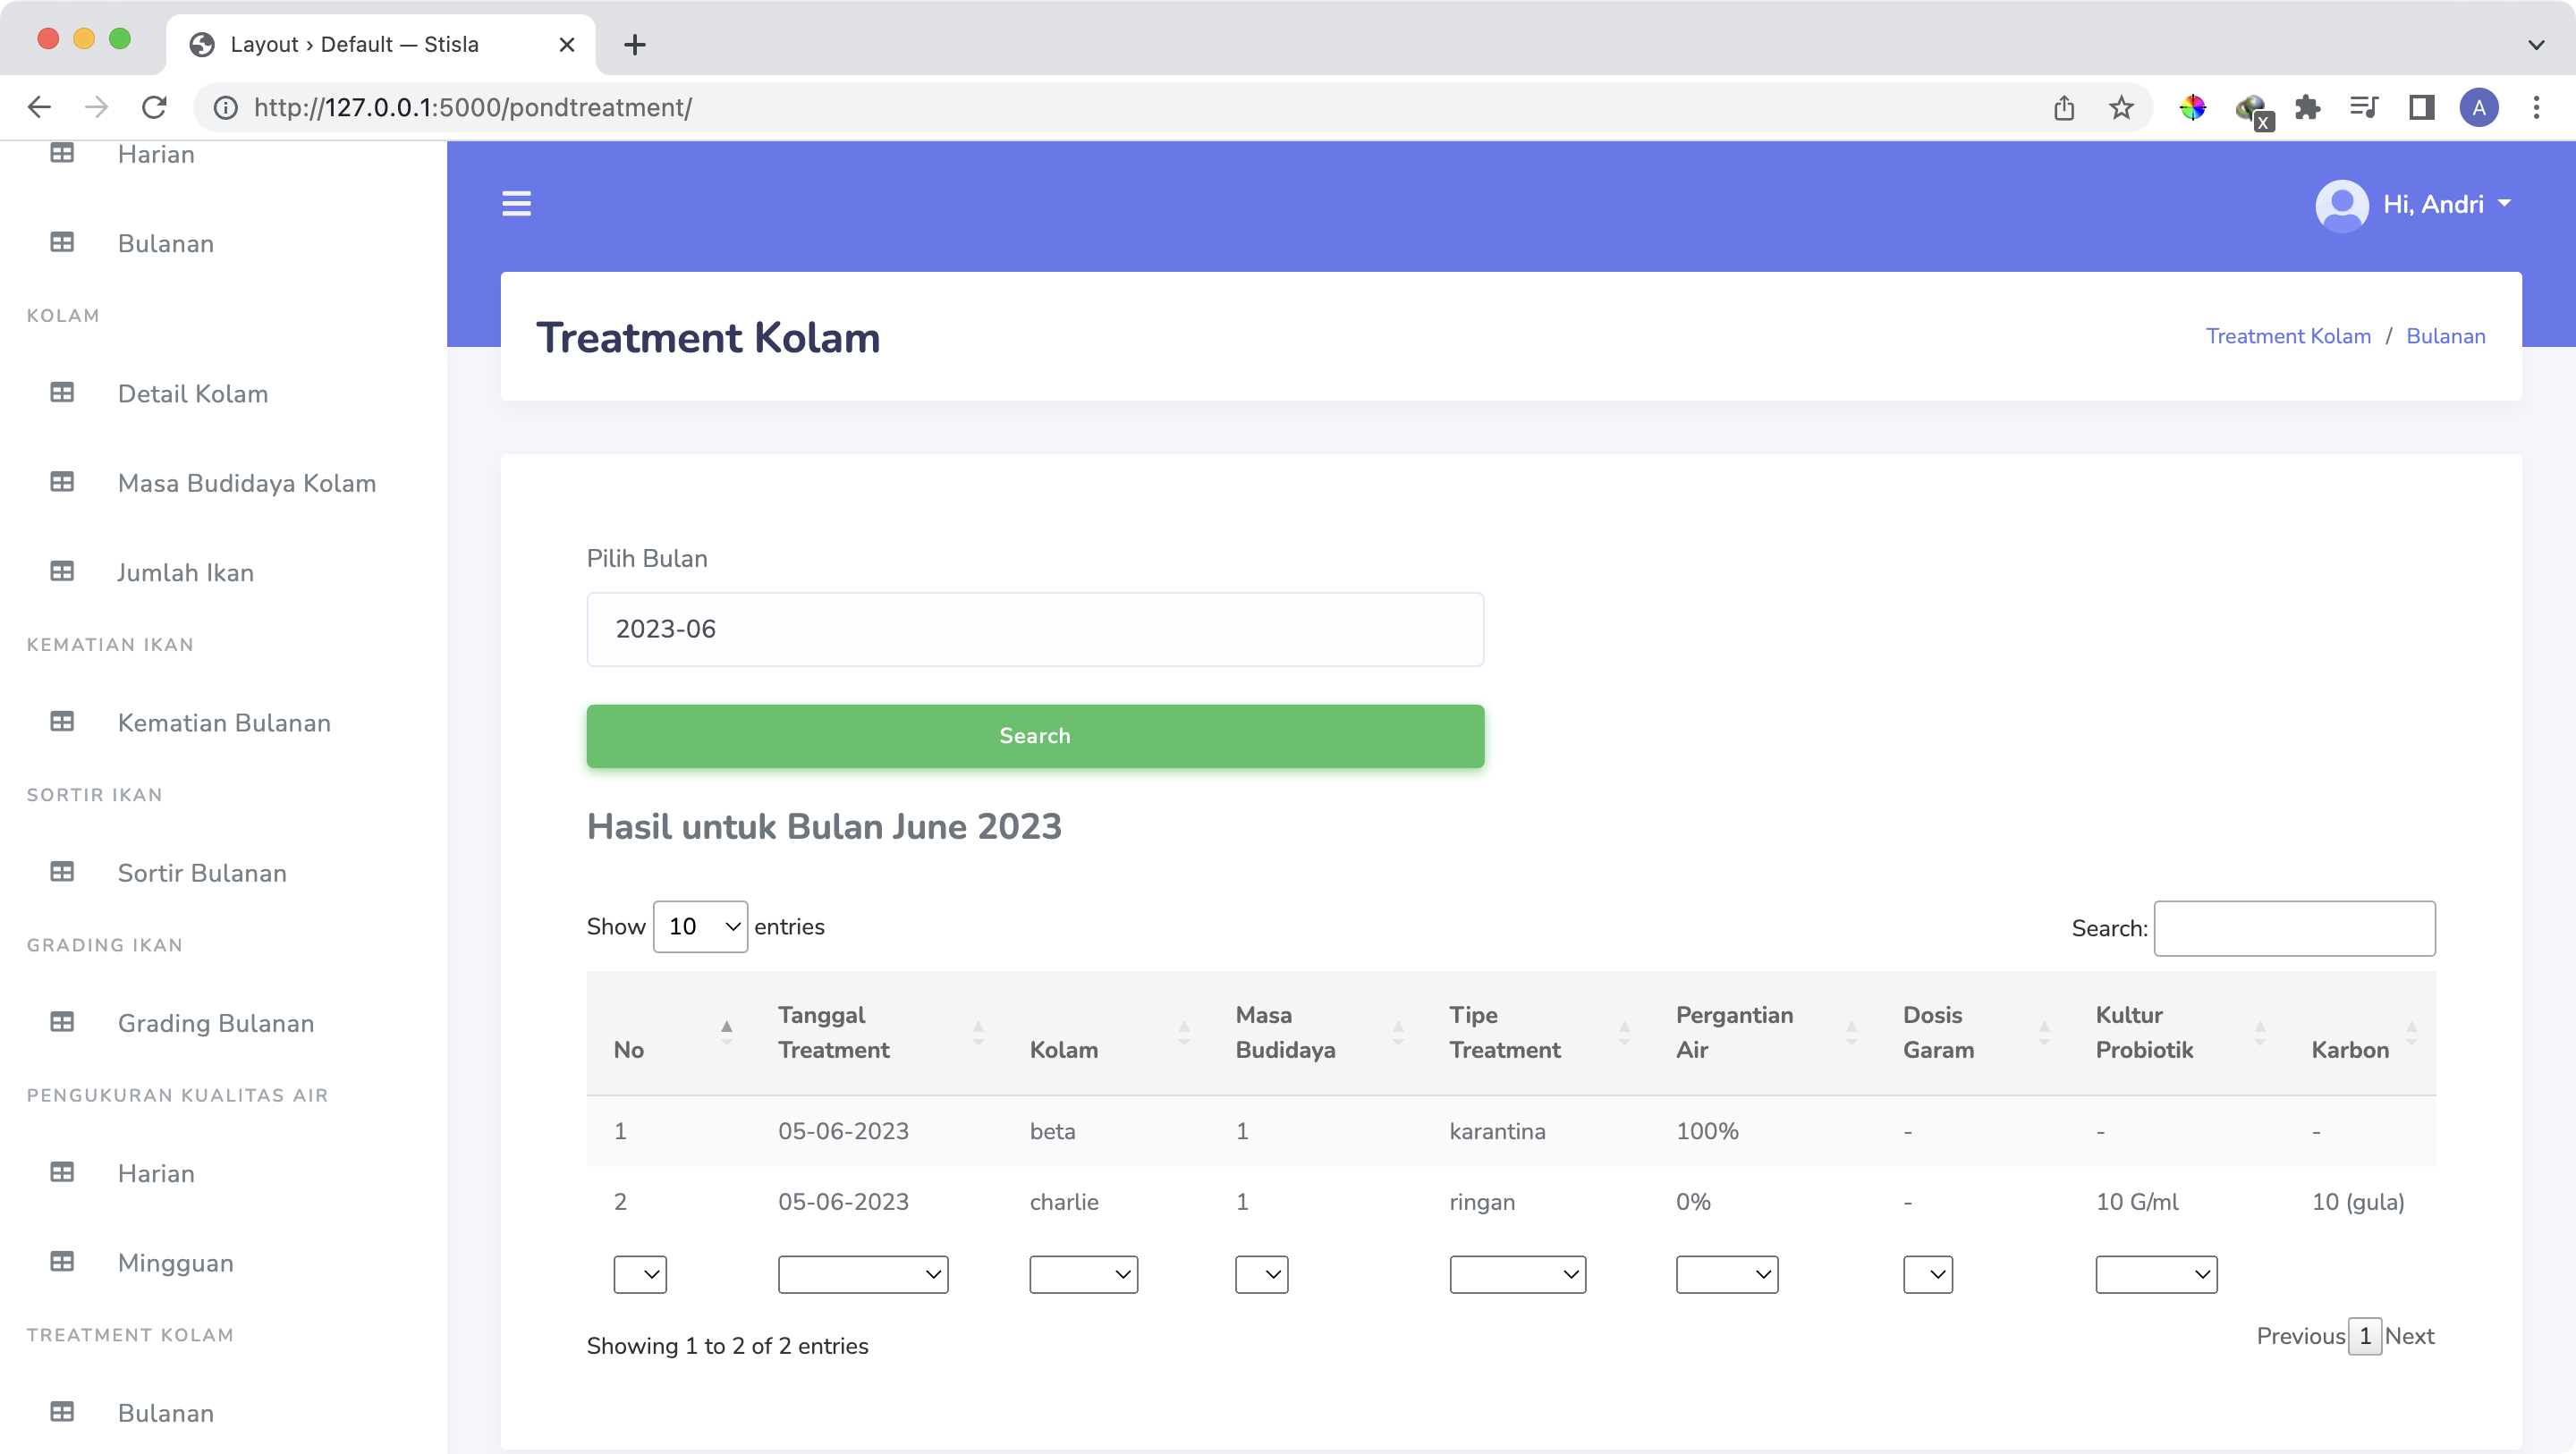
\includegraphics[width=1\textwidth]{gambar/Sprint10/view/view_rekap_treatment_kolam}
	\caption{View list treatment kolam perbulan}
	\label{fig:view_list_treatment_kolam_perbulan}
\end{figure}




\end{enumerate}